\section{Summary of the immersed boundary method}

Consider a $d$-dimensional ($d=2$ or 3) rectangular domain $\Omega$, which is
filled with a viscous incompressible fluid with constant viscosity $\mu$ and
density $\rho$, and contains an immersed elastic structure, $\Gamma$. The
structure is impermeable to the fluid and moves at the local fluid velocity, is
deformed by this motion, and imparts a force on the fluid. Otherwise, the
interface is treated as part of the fluid. 

The fluid velocity, $\vec{u} = \vec{u}(\vec{x},\,t)$, is governed by the
incompressible Navier-Stokes equations for a Newtonian fluid,
\begin{gather}
    \label{eq:ins-momentum}
    \rho(\vec{u}_t + \vec{u}\cdot\grad\vec{u}) = \mu\Delta\vec{u} - \grad p + \vec{f}, \\
    \label{eq:ins-incompressibility}
    \grad\cdot\vec{u} = 0,
\end{gather}
where $p$ is the hydrostatic pressure and $\vec{f}$ is the elastic force
density. This is a set of $d+1$ equations in $d+1$ unknowns: the $d$ components
of $\vec{u}$, and $p$. The equations are written relative to the Eulerian
frame, so that the coordinates $\vec{x}$ are independent variables. Quantities
in the Eulerian frame are written in the lower case Latin alphabet.

Let $\vec{X}=\vec{X}(\vec{\theta},\,t)$ represent a parametrization of the
Cartesian coordinates of an immersed interface with material coordinates
$\vec{\theta}$ at time $t$. Let $\mathcal{E}[\vec{X}]$ be the energy density
functional for the elastic interface material. The elastic force density is
computed by evaluating the Fréchet derivative of $\mathcal{E}$,
\begin{equation}
    \vec{F} = -\delta \mathcal{E}[\vec{X}],
\end{equation}
where $\delta$ represents the first variation. Upper case Latin letters
represent Lagrangian quantities and are functions of $\vec{\theta}$ and $t$.

To couple the fluid and interface, we employ the Dirac delta function,
$\delta(\vec{x}-\vec{X}(\vec{\theta},\,t))$. Analytically, the fluid-interface
interactions can be written
\begin{gather}
    \label{eq:interpolation}
    \dot{\vec{X}} = \int_\Omega \delta(\vec{x}-\vec{X}) \vec{u}(\vec{x},\,t)\d\vec{x},\ \text{and} \\
    \label{eq:spreading}
    \vec{f} = \int_\Gamma \delta(\vec{x}-\vec{X})\vec{F}(\vec{X})\d\vec{X},
\end{gather}
where $\dot{\vec{X}}$ represents the derivative of $\vec{X}$ with respect to
$t$. [@eq:interpolation] is called interpolation, and the result of the
right-hand side is the fluid velocity at $\vec{X}$; namely, $\dot{\vec{X}}
= \vec{u}(\vec{X},\,t)$. [@eq:spreading] is called spreading, because while
$\vec{F}$ has units of force per unit \emph{area} on $\Gamma$, $\vec{f}$ has
units of force per unit \emph{volume} in $\Omega$. The force $\vec{F}\d\vec{X}$
over area $\d\vec{X}$ is ``spread'' to the force $\vec{f}\d\vec{x}$ over volume
$\d\vec{x}$. 

Each of the fluid equations is discretized on a regular grid of spacing $h$ so
that $\Omega$ is divided into cubic cells of side length $h$. The grids can be
collocated or staggered. Because of the checkerboard instability (see, e.g.,
[@Wesseling:2001ci]) in solving the Navier-Stokes equations on collocated
regular grids, we will assume that the grids are staggered. This means that
different components of a single Eulerian vector quantity, such as $\vec{u}$,
might be evaluated at different locations. However, corresponding components of
vector-valued Eulerian quantities, and those of $\vec{u}$ and $\vec{f}$ in
particular, are assumed to be discretized on the same grid. A fixed Lagrangian
point may reside in different grid cells for each different grid. The set of
Eulerian grid points for a grid will be denoted $\Omega^h$, and define
$n_\omega = |\Omega^h|$.

The Lagrangian force density $\vec{F}$ is evaluated at a set of points,
usually a \emph{fixed} set of points in the Lagrangian variables,
$\vec{\theta}$.  The notation $\vec{X}_j=\vec{X}(\vec{\theta}_j,\,t)$ refers to
an individual Lagrangian point. The typical heuristic for distributing the
points $\vec{X}_j$ on the elastic interface is that neighboring Lagrangian
points be at most $h$ apart from one another, and often at most $h/2$ apart. We
denote the set of Lagrangian points by $\Gamma^h$ and define $n_\gamma =
|\Gamma^h|$ to be the number of Lagrangian points.

\begin{figure}[thb]
    \centering
    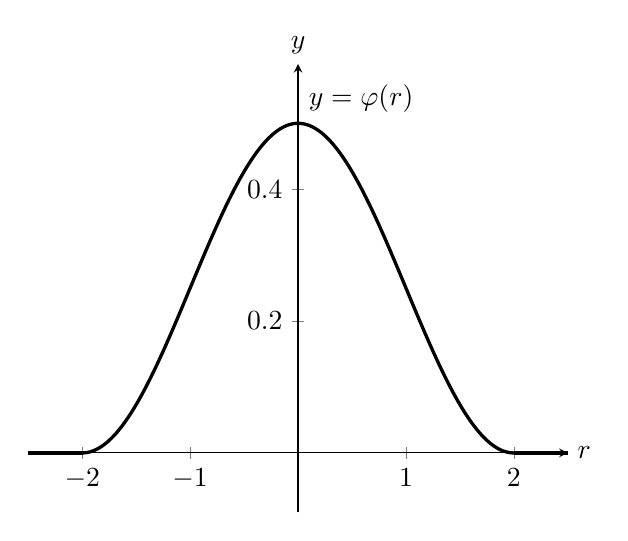
\begin{tikzpicture}
        \begin{axis}[ymin=-0.09, ymax=0.59, xmin=-2.5, xmax=2.5, axis lines=center, xlabel={$r$}, ylabel={$y$}, xlabel style={right}, ylabel style={above}, smooth, no markers]
            \addplot[samples=400, domain=-2: 2, very thick, black] {0.25 * (1+cos(90*x))} node[midway, above right] {$y=\varphi(r)$};
            \addplot[samples=400, domain=-3:-2, very thick, black] {0};
            \addplot[samples=400, domain= 2: 3, very thick, black] {0};
        \end{axis}
    \end{tikzpicture}
    \caption{%
        A compactly-supported approximation to the Dirac delta function. The
        quantity $r$ is the difference in position of an Eulerian and
        a Lagrangian point in units of grid spaces. For $r\in[0,\,1)$, only
        $\varphi(r-2)$, $\varphi(r-1)$, $\varphi(r)$, and $\varphi(r+1)$ are
        nonzero for points spaced 1 apart.
    }
    \label{fig:1d-kernel}
\end{figure}

The singular [integrals @eq:interpolation;@eq:spreading] do not lend themselves
easily to evaluation. In particular, it is unlikely that Lagrangian points and
Eulerian grid points will coincide. For a regular grid with spacing $h$, we
replace the Dirac $\delta$-function with a regularized kernel, $\delta_h$,
which is a Cartesian product of one-dimensional kernels,
$h^{-1}\varphi(h^{-1}x)$. One choice for $\varphi$ is shown in [@fig:1d-kernel]. 

A single step of the IB method proceeds roughly as follows:
\begin{enumerate}[label=(\texttt{\alph*})]
    \item interpolate $\vec{u}^n$ to $\vec{X}^n$ to get $\vec{U}^\ast$,
    \item predict data site positions $\vec{X}^\ast = \vec{X}^n + \alpha k\vec{U}^\ast$,
    \item compute Lagrangian forces $\vec{F}^\ast$ using positions $\vec{X}^\ast$,
    \item spread $\vec{F}^\ast$ from $\vec{X}^\ast$ to get $\vec{f}^\ast$,
    \item solve for updated velocities $\vec{u}^\ast$,
    \item project $\vec{u}^\ast$ into space of divergence-free vector fields to
        get $\vec{u}^{n+1}$,
    \item interpolate $\vec{u}^{n}$ to $\vec{X}^{n}$ to get $\vec{U}^{n+1}$, and
    \item update $\vec{X}^{n+1} = \vec{X} + k \vec{U}^{n+1}$.
\end{enumerate}
We group these steps into 3 categories: the purely Eulerian
(\texttt{e}) and (\texttt{f}); the purely Lagrangian (\texttt{b}), (\texttt{c}),
and (\texttt{h}); and the Euler-Lagrange coupling (\texttt{a}), (\texttt{d}),
and (\texttt{g}). The description of the methods are divided according to these
categories.
